\documentclass{sig-alternate-10pt}
%\input{nsfformat.sty}

%\usepackage{url}
\PassOptionsToPackage{hyphens}{url}\usepackage{hyperref}
\usepackage{wrapfig}
\usepackage{multirow}
\usepackage{times}
\renewcommand{\sfdefault}{phv}
\renewcommand{\rmdefault}{ptm}

%\usepackage[compact]{titlesec}

\usepackage{graphicx}
\usepackage{subfigure}
\usepackage{stfloats}
\usepackage{listings}

\renewcommand{\baselinestretch}{0.90}

\usepackage{fancyvrb}
\usepackage{fixltx2e}
\fvset{framesep=2mm,fontsize=\scriptsize,framerule=.1mm,numbersep=1mm,commandchars=\\\{\}}
\usepackage[usenames,dvipsnames]{color}

\newenvironment{packed_enum}{
\begin{enumerate}
  \setlength{\itemsep}{1pt}
  \setlength{\parskip}{0pt}
  \setlength{\parsep}{0pt}
}{\end{enumerate}}

\newenvironment{packed_item}{
\begin{itemize}
  \setlength{\itemsep}{1pt}
  \setlength{\parskip}{0pt}
  \setlength{\parsep}{0pt}
}{\end{itemize}}

\newcommand{\eg}{\hbox{\em e.g.}}
\newcommand{\ie}{\hbox{\em i.e.}}
\newcommand{\cf}{\hbox{\em cf. }}
\newcommand{\etal}{\hbox{\em et al.}}
\newcommand{\etc}{\hbox{\em etc.}}

\newcommand{\sysname}{Sensibility Testbed\xspace}

\newif\ifrev
%%%%%%%%%%%%%%%%%%
% COMMENT OUT NEXT LINE TO HIDE TODOs
\revtrue
%%%%%%%%%%%%%%%%%%

\ifrev
  \newcommand{\yanyan}[1]{{\color{blue} [Yanyan: #1]}}
  \newcommand{\cappos}[1]{{\color{red} [Justin: #1]}}
  \newcommand{\albert}[1]{{\color{magenta} [Albert: #1]}}
\else
  \newcommand{\yanyan}[1]{}
  \newcommand{\cappos}[1]{}
  \newcommand{\albert}[1]{}
\fi

\title{Reducing Mobile Experimentation Risks with \\Sensibility Testbed:
Balancing Data Acquisition \\with Privacy Protection}


\author{Yanyan Zhuang$^{\dag, \ddag}$ \and Albert Rafetseder$^{\dag}$ \and Justin Cappos$^{\dag}$ \and some other author\\
$^{\dag}$New York University, $^{\ddag}$University of British Columbia}

%\email{\small\tt \{doliveir, jnavarro, femilian\}@bowdoin}

% \and \small\tt{crandall@cs.unm.edu}}



%\begin{tabular}{cccc}
%        \multicolumn{1}{c}{Daniela Oliveira} &
%        \multicolumn{1}{c}{Jedidiah Crandall} &
%        \multicolumn{1}{c}{Jesus Navarro}  &
%         \multicolumn{1}{c}{Felix Emiliano}   \\ [.5ex] 
%        \multicolumn{2}{c}{Bowdoin College} &
%        \multicolumn{2}{c}{University of New Mexico } \\ [.5ex] 
%        \multicolumn{2}{c}{{\small\tt \{doliveir, jnavarro, femilian\}@bowdoin.edu}} &
%        \multicolumn{2}{c}{{\small\tt crandall@bowdoin.edu }} &
%\end{tabular}



%}
\date{}

\begin{document}

%\smallskip

\maketitle
\setcounter{page}{1}

%\begin{quote}
%``The world is so full of a number of things'' - that it can be extremely, even hopelessly, confusing. \emph{George Smith, 1945}

%\end{quote}

%\smallskip

\begin{abstract}
%Unfortunately, the expanded use of
%these devices also has lead to increased privacy and security 
%challenges, which makes research on these devices difficult.
In this paper we present Sensibility Testbed, an experiment  
platform for advancing the use of personal mobile devices in research, 
%security and privacy measures to ensure the
while ensuring the security of the mobile devices and the privacy of
the data generated. 
%The use model of Sensibility Testbed is
%unique in that it (1) manages how device owners make their
%devices accessible to the research community, and (2) offers
%
Sensibility Testbed's platform design not only encourages reusing 
experiment code and infrastructure, but also saves effort on 
recruiting participants and managing a deployment. 
Furthermore, Sensibility Testbed maintains device safety and privacy of 
participants. Experiment code runs in isolated sandboxes to 
prevent inadvertent or malicious bugs. Access 
to sensor values is mediated according to the policies 
set by the institutional review board of the researcher's 
university or institution. 
%using a combination of blurring and rate-limiting. 
This allows Sensibility Testbed to cater to a wider range of 
participants than prior mobile testbeds. 
%beyond that of previous campus-only,
%incentivized testbeds, thereby adding to the diversity of the
%installed base in terms of participating devices, OS software
%versions, network operators, participant demographics, countries,
%etc.
%
%experiment measures to researchers that allow them to collect
%data from remote mobile devices without rendering these devices
%at risk. 
%					
%Sensibility Testbed provides privacy mechanisms to protect
%device owners' privacy by mediating data access according to
%researcher's IRB policies. The testbed also uses security
%measures to prevent any inadvertent or malicious bugs in
%experiment code and thus protects the devices. 
Therefore, Sensibility
Testbed allows safe research without rendering devices
vulnerable, and lowers the barriers for researchers to perform
research experiment on end users' mobile devices.

\end{abstract}

\section{Introduction}

End-user mobile devices, such as smartphones and tablets, have become
indispensable gadgets in people's everyday life. %One study, conducted
%in 2015 by the Pew Research Center
Research has shown that nearly two-thirds of
Americans own a smartphone, and 19\% of them
%in that group observed that 
use the phone as their only means of staying connected~\cite{phone2015}. 
For many people, these devices have become the dominant way they
interact with others, and with the physical world.

Given the sheer number of these devices and the increasing
sophistication of their features,
the value of smart devices as data collection vehicles for government,
university, or corporate studies continues to grow. Since
these devices have embedded GPS,
accelerometers, cameras, and microphones, they can generate valuable
data for such studies as determining noise levels within an urban
neighborhood~\cite{kardous2014evaluation}, detecting approaching 
earthquakes~\cite{faulkner2011next}, or studying traffic
patterns at particular intersections~\cite{zhuang2011time}. Accessing 
devices in a home network can help providers improve the service 
quality~\cite{sundaresan2011broadband}. Testing applications on remote
devices allows developers to better understand how applications 
perform in diverse environments, enabling improvements in 
performance~\cite{ravindranath2012appinsight}. 
%For instance, some platform APIs change their behavior depending 
%on the battery level of the device~\cite{battery}. 
%Without remote access battery life, these APIs can not guarantee basic function efficiency.
%Even being able to
%remotely assess how much life is left in the battery of a device can
%help platform APIs deliver better service to its
%customers~\cite{battery}.
%
As a result, there have been initiatives within the network
community to study mobile devices (e.g.,
Mobilyzer~\cite{nikravesh2015mobilyzer}), and in the systems community
to deploy new services and test research prototypes (e.g.,
Phonelab~\cite{phonelab, nandugudi2013phonelab}). However, personal devices
remain largely underused because of two interrelated challenges:

\begin{itemize}\setlength\itemsep{0em}
\item The risk research studies pose to the privacy of \textbf{device 
owners}, and 

\item The difficulties \textbf{researchers} have
%\cappos{Do you mean obtaining access due to IRB constraints?  What does 
%"securing" mean here?}
obtaining access to devices due to the restrictions set by Institutional Review 
Boards, and using data gathered in a responsible and ethical manner. 
\end{itemize}
					
For device owners, privacy and security threats to mobile devices have
increased dramatically over the years as potential attackers seek
to take advantage of the rich functionality that %and user experience that
sensors\footnote{\scriptsize In this work, we broadly define sensors
as the hardware components that can record phenomena about the
physical world, such as the WiFi/cellular network, GPS location,
movement acceleration, etc.} on mobile devices can provide.
Data acquired through a smartphone's GPS,WiFi
connections, or Bluetooth pairing history can be highly personal,
exposing sensitive information, such as where a person lives or 
shops~\cite{han2012accomplice}. Seemingly benign applications, 
such as popular online games downloaded to mobile devices, can
leak data, such as the model number of the device, or the age, gender, 
or location of its owners~\cite{AngryBirds}. Furthermore, running experiment code poses 
a risk to the operation of the device itself through potential exposure 
to bugs and other vulnerabilities. 
%It can also seriously interfere with battery life, if the device 
%is accessed too often.

For researchers, the challenges are equally formidable. 
Researchers' experimenters are under the governance of Institutional 
Review Boards (IRBs)~\cite{irb} that
review all experimental protocols involving human subjects,
and set a strict set of procedures that any researcher working under
the aegis of the institution is required to follow. These include
careful control over the collection and storage of data to ensure the 
privacy of subjects is preserved. It falls on the researcher to enforce 
these policies, and the process must be repeated every time he or 
she starts a new project. The experimenter must also recruit device 
owners willing to volunteer their devices for testing, a process that 
is time-consuming. Moreover, experimental setup and results cannot 
easily be shared with other researchers. 
%As a result, each research group has to repeat the process of 
%infrastructure setup, and policy implementation \cappos{what 
%is this?} for each experimental deployment.

Due to these concerns, experimental testbeds either do not use data 
from real participants (using archived traces like 
in~\cite{kapadia2008anonysense}) or use data collected 
from a tightly controlled, non-representative subset of participants.
%such as PhoneLab, have been established to provide a platform for 
%running apps on smartphones. 
%PhoneLab recruits participants by giving them free
%smartphones and reduced data plans in exchange for their commitment to
%use the phones as their personal devices. 
%PhoneLab then runs Android apps on the devices and collects data. 
For example, some testbeds deal with both
the recruitment and privacy issues by choosing to select participants
from an internal group, such as faculty working with their students
and colleagues~\cite{hao2013isleep, wang2012no, wang2013sensing}. 
Other testbeds require researchers obtain IRB approval prior to using the
testbed, but provide no technical measures for IRB policy 
enforcement~\cite{phonelab, nandugudi2013phonelab}. 
These mechanisms still fall short, as they do not 
relieve the burden on the researchers to ensure the privacy of the
device owner and to enforce IRB policies. 
%Since the present network testbeds do not yet have a systematic way 
%to provide these protections, there is limited protection for the device 
%owners. 
%Research has shown that most people usually do not understand 
%the basics of privacy, or the implication of granting device
%permissions~\cite{camp2015respecting}. Therefore, if the testbed does 
%not safeguard the security of devices, no matter what 
%advantages participants may receive, their devices are still at risk.
%\cappos{I miss the point of this paragraph in the rest of the narative...}

In this work, we introduce Sensibility Testbed~\cite{sensibility,
zhuang2015privacy}, an Internet-wide mobile testbed that 
%represents an important first step towards 
lowers the technical barriers to research on personal mobile
devices without lowering the ethical standards of the research
institution~\cite{zevenbergen2013ethical}.  
%\cappos{I would instead emphasize 
%that it streamlines IRB since it acts as a middle man for experimenters and 
%participants.  The paragraph here seems to wander to me (e.g., where do we
%discuss ``making prototyping faster'' again?), but eventually comes
%to this point anyways.}
The new testbed streamlines the IRB process for researchers as it acts 
as an intermediate between researchers and device owners. 
%makes experiment prototyping faster, the remote
%control and management of devices easier, and the running of
%experiment code more secure in a number of ways. 
Researchers provide their policy specification to the testbed, and 
the testbed recruits participants and implements the policies on researchers' 
behalf. This model 
makes experiment prototyping faster and more secure in a number of ways. 

First, \sysname provides better protection against invasion of privacy by carefully controlling
access to device sensors. The testbed employs a stringent set of
policies as to which sensors can be accessed, and these
policies are customizable to each researchers' IRB policies. 
%This serves as a template for researchers to parameterize their 
%experiment. 
Second, the testbed infrastructure automatically implements
the IRB policies on end-user devices, through the use of \textit{blurring 
layers} in a secure sandbox. Each blurring layer mediates the access to 
a sensor by limiting the precision of data generated by it, by 
regulating the frequency that the sensor can be accessed, or both. Policy thus
can be easily enforced at the end-user devices by the testbed 
infrastructure. In addition, 
the testbed's secure sandbox provides both security and performance 
isolation, and ensures experiment code cannot harm the devices of 
volunteers. Due to these privacy and security mechanisms, 
the enrollment process for volunteer device owners is as
simple as a one-time download and install of an app. The testbed thus
builds and maintains a pool of willing participants for researchers to
choose from, eliminating the time-consuming process of recruitment.


The contributions of this work are as follows:

\begin{itemize}\setlength\itemsep{0em}
%\item We identify the issues that have prevented successful implementation
%of experiments on remote user devices, including potential damage to
%devices from experiment code, the risk of privacy invasion, and the
%administrative challenges faced potential researchers. 

\item We introduce Sensibility Testbed as a flexible and secure platform for
conducting experiments on Android devices that addresses the
concerns above, including automatically obtaining and enforcing 
institution-mandated IRB policies. \sysname identifies potential 
risk of privacy invasion and alleviates administrative 
challenges faced by potential researchers.

\item We describe the unique features of Sensibility Testbed, which include 
controlled sensor access through the development of blurring layers that are
highly customizable.

\item We evaluate Sensibility Testbed's effectiveness in
protecting device owners' privacy and find that nearly 85\% of
security and privacy issues present in previous projects using 
mobile devices were addressed by the default policies.
\cappos{I'm not sure that the quantitative parts of the analysis are 
what we want to emphasize at this point.  If we do this, we need to set it 
up differently.  I would also wonder how useful this is if the number isn't
100\%...}
\jill{i think the contributions should be: 
1. ST streamlines the process of IRB policy enforcement, which makes experiments safer for device owners and easier for researchers who no longer have to recruit mobile device participants 
2. ST allows researchers to run multiple experiments using ST without having to obtain an IRB and rewrite code enforcing the policies of the IRB for each experiment.
3. controlled sensor access through blurring layers
4. perhaps something here about default policies for protecting the privacy of device owners as an extra precaution}
\end{itemize}

The rest of this paper is organized as follows. In Section~\ref{sec-motivation} we
present background information about several key concepts of \sysname. 
%that are critical to understanding how Sensibility Testbed works and how its use can benefit both researchers and device owners. 
Section~\ref{sec-overview} offers an overview of the design principles 
%including a description of its key components and a simplified look at 
and the operation of the testbed. The architecture of the Sensibility Testbed 
is reviewed in Section~\ref{sec-design}, and Section~\ref{sec-policy} 
presents the detailed implementation of the architecture. 
%while Section offers a detailed walkthough of the program in operation. 
Section~\ref{sec-eval} provides experimental results to prove the
viability of Sensibility Testbed in enforcing privacy policies, while
Section~\ref{sec-limitation} examines challenges and current limitations. 
In Section~\ref{sec-related} we review related work,
%in protecting the privacy of data on mobile devices, 
and we share our concluding thoughts in Section~\ref{sec-conclude}.



\section{Motivation and Background}\label{sec-motivation}


 In this section, we present some background information that served as the building blocks of the  design and deployment of Sensibility Testbed. First, we offer the motivations behind its development: the desire to balance the benefits of such research with the very real privacy risks that could potentially occur if a device owner allows access to his/her device. Next, we look at one solution to the problem?the collecting of proximate versions of data through the use of blurring layers. Third, we talk about the traditional role of IRB in research involving human subjects and how Sensibility Testbed can ensure these protections extend to data accessed remotely. Lastly, we look at Sensibility Testbed?s sensor default policies, which automatically closes off access to sensors which have the highest risk for violating the privacy of device owners.


%Apps can post tweets to a 
%user's Twitter account without asking for permission~\cite{tweet}. 
Motivation: Overcoming the Risks of Accessing Sensor Data

Having access to data from the enormous number of smartphones 
in use today could be tremendously valuable to the research 
community. The sheer numbers of these devices, coupled with the fact that research on these devices do not incur high maintenance costs, makes their potential as information gathering instruments almost limitless. 
%As a result, device owners 
%are aware that running apps on their smartphones can raise privacy 
%and security risks. 
However, for the research community, accessing this data depends on its 
ability to provide strong protection to device owners from privacy 
and security breaches. In seeking solutions to this problem, we started with a few key ideas. The first is that device owners themselves may not fully understand the implications of granting access to a particular type of sensor or resource~\cite{felt2012android}. It is 
therefore challenging to conduct research on end-user devices
in compliance with ethical standards, without some type of organized approach to enforcing those standards.~\cite{zevenbergen2013ethical). In addition, a major reason for the prevalent privacy breaches on many mobile systems, including Android, is that 
only a sub-set of sensors like GPS and bluetooth are considered risky, 
and therefore have their access mediated~\cite{android-sec}. Other sensors 
such as accelerometer, gyroscope, etc., 
%are considered to be innocuous, 
require no permission to access, thus leaving them open to attack. Therefore, with Sensibility Testbed, both the inclusion of IRB restrictions (discussed later in this section), and the need to restrict or limit access to a wider range of sensors were both incorporated into the design.

\textbf{Restricted data access and privacy protection}
%Despite these risks of using sensors, 
Another concept important to our design is that generalized data that does not directly violate the privacy of the device owner can still be valuable. Studies have indicated that 
sensor data can be accessed without compromising device 
owners' privacy or sacrificing service functioning.
A recent research study shows that more than half of the 
surveyed individuals had no problem in supplying imprecise 
sensor data from their personal devices~\cite{fawaz2014location}. 
Most participants could accommodate some inevitable loss of application 
functionality, as long as their privacy was protected. Those surveyed
applications ranged from location-based search (e.g., Yelp), social 
network apps, to gaming and weather forecasting apps. 
Researchers thus have proposed 
substituting mocked~\cite{beresford2011mockdroid} or 
anonymized~\cite{zhou2011taming} data in place of real data. 
For example, in location-based services such as maps, 
restaurant guides, and bus schedules, end users can still use the 
service even if a device only provides a discretized 
location~\cite{amini2011cache, krumm2007inference}. Therefore, 
though the accuracy of the data is reduced, 
the imprecise information is sufficient for a large class of services. 
%The US Federal Communications Commission requires 
%emergency rescue and 
%response teams to be able to estimate a 911 wireless emergency 
%caller's position with an accuracy of 125~m~\cite{gruteser2003anonymous, 
%reed1998overview}. \yanyan{too many examples?}

Based on these facts, we decided that restricting 
the amount of data accessible, such as reducing the precision or 
access frequency, offered an effective privacy protection mechanism to 
provide to end users. In this work, we coin the term \textit{data blurring}
as our privacy protection mechanism. This concept, explained in detail in section 4.2, automatically limits the amount of detailed information the device sensors will relay to the person running the experiment.
%where each data access
%policy is codified as a blurring layer, and different policies are
%customized by loading individual blurring layers in order.

\textbf{IRB policies: Guiding Ethical Behavior}
%On the other hand, research institutions have also designed a 
%protocol based on the \textit{institutional review board (IRB)}, 
%to assess the ethics of a researcher's project, and review its methods. 
Institutional Review Board serve as the ethical watch dogs for college, universities, government agencies, and other research institutions. It is the job of these boards, also known as an independent ethics committee (IEC), ethical 
review board (ERB), or research ethics board (REB), 
t to approve, monitor, and review 
research involving human subjects~\cite{irb} These groups require all researchers working under their aegis to submit the protocols of their studies with an aim to protecting not only the physical and mental well-being of subjects, but also to protect any information about these individuals generated over the course of the study. Since privacy protection of collected data become a bit more difficult when dealing with remote subjects, another issue we sought to address with Sensibility Testbed is to 
relieve the individual researcher of the need to manually enforce 
the restrictions set by his or her institution's IRB.
Sensibility Testbed automates, and therefore ensures adoption of these policies. Although many current network 
testbeds require that researchers obtain IRB approval before conducting
an experiment on the testbed, these platforms do not provide a guarantee 
for IRB policy compliance.~\cite{nandugudi2013phonelab, nikravesh2015mobilyzer}. 
%In the case of PhoneLab, 
%it requires experimenters to obtain IRB approval. However, 
%Similarly, Mobilyzer~\cite{nikravesh2015mobilyzer} provides a 
%measurement library that can be included in Android apps. 
%and requires explicit user consent. 
Therefore, there is no guarantee that an 
experiment will be compliant with a researcher's IRB policies.
%promotes fully informed 
%consent and voluntary participation by prospective subjects. 

Sensibility Testbed takes any researcher's IRB policies, codifies them, and uses the aforementioned blurring layers 
 to restrict sensor access on an end-user's device to 
an institution's set access levels, making compliance automatic. 
%IRB plays a central role in defining the policies
%appropriate for research at individual institutions. Experimenters
%first obtain an IRB approval at their institution. Then with these IRB
%policies, Sensibility Testbed, as an intermediate, codifies the data access 
%regulations and enforces them at the end-user mobile devices. 
Each policy layer implements an IRB policy by substituting 
approximate data in place of explicit, raw sensor data to the experiment code, and different layers 
together can be customized to cater to various institution's 
policies and regulations. As a result, experiments 
do not collect more data than needed to provide their functionalities.


%In the domain of IRB, Alice and Bob are the participating subject, and 
%a researcher who conducts a research study on the subject, respectively.
%
%
%\textbf{Sensibility Testbed's default policies.}

\begin{table}
\scriptsize
\centering

\bgroup
\def\arraystretch{1.15}% % for table padding
\begin{tabular}{|l|c|c|c|}
\hline
\multirow{2}{*}{\bf Sensor} & 
\multicolumn{3}{c|}{\bf Default policy} \\\cline{2-4}
& {\bf LR} & {\bf MR} & {\bf HR} \\\hline

Battery (plug-in type, level, technology, etc.) & \tickmark &  & \\ \hline
Bluetooth (local name, scan mode, etc.) & & \tickmark & \\ \hline

\multirow{2}{5.5cm}{Cellular network (cell ID, area code, country code, 
operator name, etc.)} & & \multirow{2}{*}{\tickmark} & \\ 
& & & \\ \hline

Location (latitude, longitude, altitude, speed, etc.) & & \tickmark & \\ \hline
Settings (screen brightness, ringer volume, etc.) & & \tickmark & \\ \hline

\multirow{2}{5.5cm}{Motion sensors (accelerometer, 
gyroscope, magnetometer, orientation , etc.)} & & \multirow{2}{*}{\tickmark} & \\ 
& & & \\ \hline

\multirow{2}{5.5cm}{WiFi network (information about the 
currently active access point, and WiFi scan result)} & & \multirow{2}{*}{\tickmark} & \\ 
& & & \\ \hline 

%Start/stop activities & & & \xmark \\ \hline 
%Running applications & & & \xmark \\ \hline 
Camera (take pictures, record videos) & & & \xmark \\ \hline 
Intent (scan barcode, search, etc.) & & & \xmark \\ \hline 
Address book & & & \xmark \\ \hline 
Microphone (voice record) & & & \xmark \\ \hline 
SMS (send/receive messages, delete messages) & & & \xmark \\ \hline 

\end{tabular}
\egroup

\caption{\small Sensibility Testbed's default policies for sensors. LR/MR/HR
stands for low/moderate/high risk, respectively. Access is only allowed to sensors that have low to 
moderate risks (marked by \tickmark). Sensors that are highly risky are 
disabled by default (marked by \xmark).}
\label{tab:default}
%\vspace{-10pt}
\end{table}

\textbf{Sensibility Testbed's Default Policies.} %\label{sec-irb-policies}
The last unique concept Sensibility Testbed leveraged to  ensure protection of end-user security and privacy protection is that all sensors are not alike. As mentioned at the beginning of this section, failure to recognize the vulnerability of certain sensors was a key reason for privacy breaches. In designing Sensibility Testbed, default policies were set as to what types of sensors could be accessed. Even if his IRB happened to approve such a policy, there are certain sensors that the testbed's
own IRB designates as off-limits due to the high risk associated with potential breaches. 
%and for which access can be pre-approved with the
%researcher's local IRB. 
Only those sensors listed on our project 
wiki page~\cite{sensor-api} are accessible to a researcher. 
A summary of these sensors is listed in Table~\ref{tab:default}, 
with each one categorized as low, moderate or high 
privacy risk.The list of sensors that Sensibility Testbed provides are all of moderate 
to low privacy risks (marked by \tickmark), and the testbed further provides policy enforcement
(Section~\ref{sec-policy}) to protect all the sensor data. Sensors 
such as cameras and microphones that are deemed sensitive are not 
exposed to experiment code by default (marked by \xmark). Such 
classification is motivated by the Android system, where 
permissions are categorized into different protection levels~\cite{level}:
\textit{normal} permissions are automatically granted to the apps, 
\textit{dangerous} permissions are given based upon the 
user's consent, and so on. In our case, 
%we divide sensors into different risk levels, as shown 
%in Table~\ref{tab:default}. 
%Sensors with low to moderate risk are 
%allowed and protected by IRB policies. Sensors of high risk are 
%disabled by default. 
we divide sensors into different risk levels by the consequences and 
difficulties of a potential attack. If a microphone is controlled by 
a malicious party, it can be used to intelligently choose data of a 
higher value (e.g., credit card number, password) to record~\cite{zhang2015leave}. On the other 
hand, in order to infer a credit card number or password typed on a 
smartphone using motion sensors, the attack requires the installation of 
a sophisticated algorithm on the device that constantly learns about  
the patterns of data generated by accelerometer or gyroscope. In contrast,
using battery information alone is not sufficient to create a fingerprint 
for each device. Different information and mutiple occurrences need to
be pieced together to extract this data~\cite{battery-priv}. Therefore, 
compared to motion sensors, a microphone is considered a higher risk, 
and a battery is a significantly lower risk.

Although high-risk sensors are disabled, if such access  is critical to the 
study, access can be requested using a different IRB procedure. 
In this case, the research project has to go through the Sensibility 
Testbed's IRB, in addition to the researcher's IRB. 
\yanyan{if we think this is ok, then we provide specially
designed interface and policy?} \lois{following up on Yanyan's comment--If the Testbed's IRB says this expanded access is permissable, are the device owner's notified and can they opt out of this study? Otherwise, that would be a direct violation of the privacy protection you claim to give them}\lois(I did not touch these last two paragraphs because I still don't know about  the opt-out policy for individuals if this permission is given).
%Depending on the experiment description provided by the 
%researcher, the fields marked with a (*) are the ones that will be blurred.
%
%



\section{Sensibility Testbed Architecture}\label{sec-design}

The architecture of Sensibility Testbed is comprised of three main components that are critical 
to its operation, as shown in Figure~\ref{fig-arch}. In this section, we discuss each of these components in 
greater detail, describing their functions and introducing several key 
techniques that make the testbed's enhanced security possible. 

\subsection{Device Software}\label{sec-repy}

%In Sensibility Testbed, all experiments execute in a secure 
%sandbox on the end devices.
%Experimenters' code executes in a sandbox that isolates the 
%experiment code from the device host system. 
The device software of Sensibility Testbed is the only one of the three 
components that runs on end users' devices. It is divided into three 
parts: a secure sandbox called Repy (Restricted Python), a resource 
manager that facilitates the interaction between researchers and the 
sandbox, and a device manager that allows the device owner to control 
if the sandbox and resource manager can run on the device.


\subsubsection{Secure Sandbox} 
The Repy sandbox is the most important in the device software. This 
security-reviewed sandbox~\cite{cappos2010retaining} mitigates the 
impact of bugs in experimenter code by providing security isolation 
and performance isolation\footnote{\scriptsize 
This sandbox has been used successfully for more than six years in our 
prior work, the Seattle testbed~\cite{seattle}.}. 
%Instead of developing full-fledged Android apps, all 
%experiments in Sensibility Testbed are written in a language
%similar to Python, and run in a secure %Python-based
Researchers use a Python-like programming interface~\cite{repyv2}
to write experiment code, upload the code and execute it in the
sandbox on remote devices. The programming interface includes functions for networking, 
file system access, threading, locking, logging, and so on. To access sensors, 
the sandbox also has a set of sensor functions~\cite{sensors}. 
%Details about implementing the Repy sandbox for mobile 
%devices are described in Section~\ref{sec-repy-ext}.
%
%However, the current Repy sandbox does not include calls to access sensors. 
%%To obtain the sensor data, we need to extend the sandbox. 
%The extended Repy sandbox that allows sensor access  
%will be described in Section~\ref{sec-repy-ext}.
Another important feature of the Repy sandbox allows us to change the 
behavior of its programming interface, and control the 
data gathered from the device to adapt to any IRB proscribed limits. 
%For  an experiment
%that involves GPS location, a privacy policy might restrict the
%level of data granularity available to the experiment. For example, it can
%obfuscate GPS location such that it only identifies the center
%of the city that the device is located in, rather than the exact
%location. Using the same technique, 
For example, the sandbox can anonymize the IP address of a device, constrain  
the frequency of access to GPS locations, and disable
access to cameras. 
%Such privacy protection is a contribution of Sensibility Testbed, 
%which does not exist in any prior work. 
The details of policy implementation are presented in 
Section~\ref{sec-layer} and \ref{sec-nanny}.

\textbf{Security and performance isolation.}
The sandbox is the execution environment 
of all experiment code. It isolates experimenters' programs from one 
another, and prevents any of the code from harming the device 
through its strong isolation techniques. More importantly, the sandbox
provides a flexible system call interposition technique where system call behavior 
can be modified. This allows us to define and implement
different data access policies. 

Repy has a small, self-contained kernel as its trusted 
computing base (TCB). %unprivileged libraries and experiment code. 
Every system call in the TCB is strictly 
sanitized to preserve consistent behavior across different OSes, 
and to avoid uncommon corner cases that can be exploited. 
Furthermore, since the TCB is small (about 8,000 lines of code), it is 
less likely to have a kernel exploit than other more complex kernels. 
As a result, any vulnerability in an experiment 
%can at most cause compromise in the unprivileged portion of the sandbox, 
cannot escape the sandbox and perform malicious actions to 
the device system. The Repy sandbox exposes its system calls for 
accessing resources on a device through a Python-like programming 
interface~\cite{repyv2} isolating experiment code from the kernel. 
%another way of saying this:
%Experiment code for accessing resources is contained by the 
%Repy sandbox, using its Python-like programming language interface.
This same sandbox design has been successfully running experiments as part of a network research 
testbed for more than six years, without significant operation faults or security breaches~\cite{seattle}. \yanyan{Justin thinks this statement is weak.} \lois{I don't know if this answers his concerns since the meaning is essentially the same}
%=======
%through a Python-like programming interface~\cite{repyv2}. 
%%to experiment code for accessing resources on a device. 
%%another way of saying this:
%%Experiment code for accessing resources is contained by the 
%%Repy sandbox, using its Python-like programming language interface.
%This same sandbox design has been successfully running experiments 
%as part of a network research testbed~\cite{seattle} for more than six 
%years, with no report of operational faults or security breaches. 
%>>>>>>> yyzhuang/master

In addition to security isolation,
%The sandbox exposes a programming 
%interface to experimenter programs to access 
%resources on the device. 
the sandbox provides performance isolation by
%by using OS hooks to monitor and control the amount of 
%CPU and memory used by a sandboxed program. To restrict 
%other resources, such as network and disk I/O, the sandbox 
interposition on system calls~\cite{garfinkel2003traps} that 
use resources, such as network and disk I/O, and preventing 
or delaying the execution of these calls if they exceed 
their configured quota. 
%As a result, this sandbox limits 
%what a sandboxed program can do. For example, 
This isolation means the sandbox can set access limits. For example, 
reading from and writing to the file system can
only occur in a per-experiment directory, sending and receiving
data via the network interface cannot exceed a configured rate, and 
CPU, memory and battery consumption cannot exceed a set level.
Therefore, the sandbox isolates the experiment program from 
the rest of the device. Due to this isolation, different researchers 
can run experiments on different sandboxes on the same device, 
without any interference between the experiments.

\begin{figure}
\center{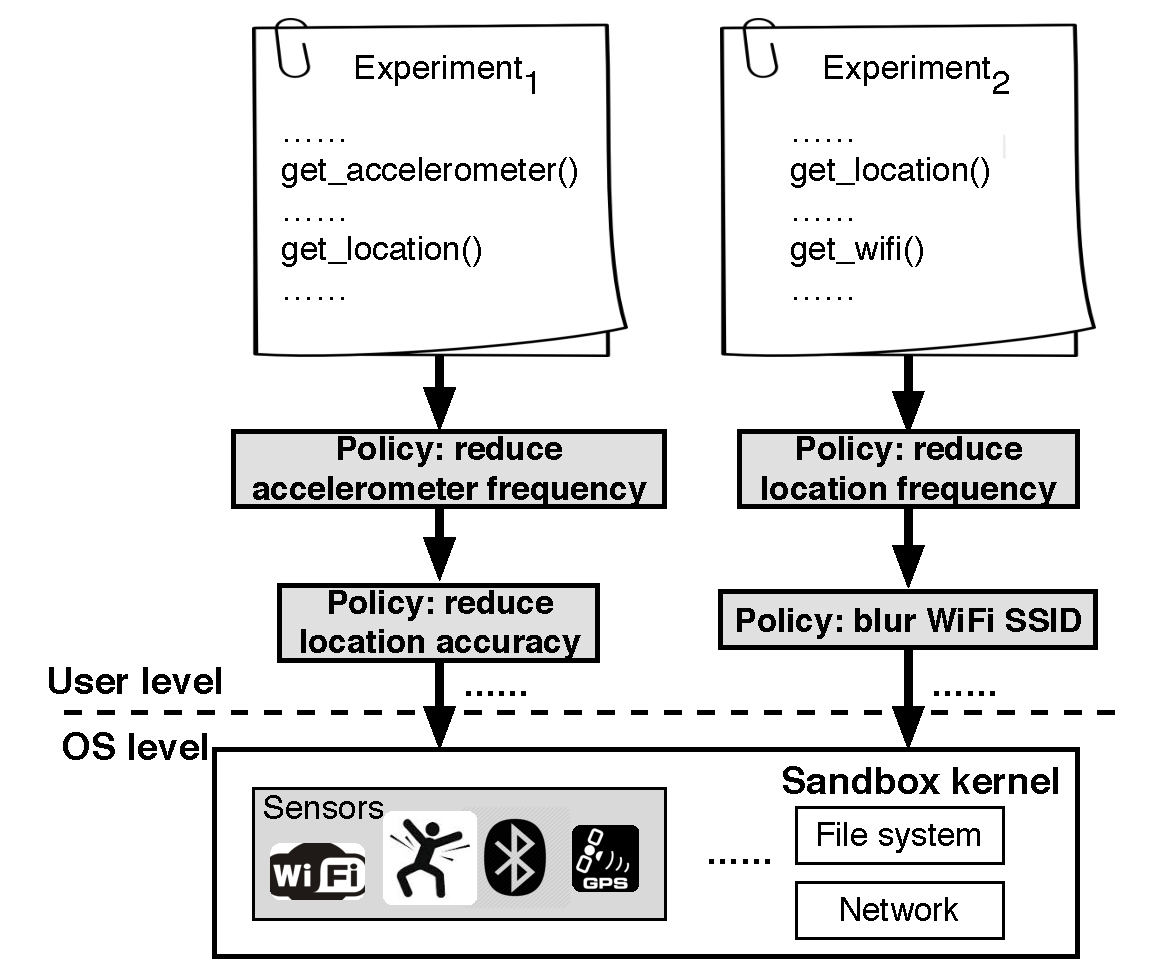
\includegraphics[width=0.9\columnwidth]{figs/blur.pdf}}
%\vspace*{-20pt}
\caption{\small Policy stack demonstrating how Sensibility Testbed implements blur policies.
\label{fig-blur}}
\end{figure}

\textbf{Policy stack.}
In Sensibility Testbed, privacy policies are implemented as blurring layers, with each layer acting as a 
reference monitor in the sandbox~\cite{ref} to enforce an access 
control policy over each sensor. Using the sandboxing 
technique in our prior work~\cite{cappos2010retaining}, we are able to
interject code to control the behavior of sandbox functions, or 
system calls. A sensor access policy can (1) reduce 
the precision of the raw sensor data returned from a device, such
as returning the location of a nearest city rather than the device's exact location, and (2) restrict 
the frequency of access to a sensor, such as the polling rate of a gyroscope or
an accelerometer, to avoid password interference~\cite{michalevsky2014gyrophone}.

%and (3) disable  
%access to a certain sensor in sensitive situations, such as 
%turning off a camera when a device is in a residential or work area.
%Implementation of the last policy is still ongoing, so this paper will mainly address
%how blurring layers allow for the execution of the first two types of policies. 

%The sandbox kernel determines how IRB policies are implemented by affecting system calls. It can
%interpose on a call and modify the data returned, or control the frequency with which a call can be made over
%a period of time. 

%Different policies implemented can be stacked in tandem to 
%control different sensor accesses, like in Figure~\ref{fig-blur}.
%As mentioned above, Bob provided his IRB policies through our clearinghouse.
%Before Bob runs his experiment, the clearinghouse loads the access policies and instructs the sandbox on Alice's device to
%restrict sensor access accordingly. 
%
%Using the \path{get_location()} call as an example, 
%when Bob's code requests location data from Alice's device, the Repy sandbox first
%invokes the location-related Android code. 
%%(line 10 in Figure~\ref{fig-getlocation}). 
%When the location data is returned, according to Bob's IRB policy
%indicates that the returned location coordinates should be blurred to the nearest city to Alice's
%device, instead of her actual location. As a result, 
%For example, the sandbox returns a perturbed location that is less accurate, 
%%Furthermore, as Bob's IRB policy disallows collecting information about cell tower IDs, 
%%blocks any access to cell IDs, 
%%by another policy. Similarly, other information
%blurs a WiFi SSID to a hashed string, and restricts the frequency to access a
%gyroscope to prevent inferring passwords~\cite{michalevsky2014gyrophone}, and so on. 
Each policy is a blurring layer, which defines either of the above
two categories of policies. Different sets of policies can be customized 
according to the regulations set by IRB, through loading 
individual blurring layers in order, as a policy stack. In each stack, 
a lower layer is the ancestor of a higher layer. Every layer inherits 
the policy defined by its ancestor layers, with the exception of the lowest layer. 
%Each blurring layer is untrusted by its ancestor layers, 
%but is trusted by its descendant layers. \yanyan{maybe cut this.}
The lowest blurring layer with no ancestors is the 
Sensibility Testbed's sandbox kernel. The experiment program runs at the top 
of the policy stack, thereby inheriting all the policies defined by the
lower layers, as shown in Figure~\ref{fig-blur}. 
Each policy stack acts as a set of filters for different sensors, through 
which a call must pass before a sandboxed program can
access the sensor data. 
%Different stacks can be customized for different IRB policies.


%In the following, we describe how to implement each blurring layer, 
%and use them to form a policy stack.


\subsubsection{Resource Manager} The second part of the device software, called a resource manager, 
establishes a trust relationship between a device and a researcher. It 
manages a researcher's access to the sandboxes on a device, and
controls the start and stop of the sandboxes on the device. The 
resource manager controls which researchers can access the 
sandbox on any given device, and communicates with the clearinghouse
or experiment manager. If multiple researchers have access to 
the same device, the resource manager splits the resources in the 
sandbox among the researchers, and partitions the one sandbox 
into several smaller ones. In order for the clearinghouse or a 
researcher's experiment manager to discover the sandbox on a 
device, the resource manager also contacts a lookup service that 
announces the existence of the available devices. An example is 
given in Section~\ref{sec-case1}.

\subsubsection{Device Manager} The last part of the device software is a device manager that 
allows device owners to manage the software running on their 
devices. This is the only part of device software that a device owner 
will interact with directly. With the device manager, a device owner  
can install and remove the device software, and start and stop the 
operations. The device manager also provides a user interface to 
allow a device owner to opt out of any experiment. Thus, the device 
owner has the freedom to choose what experiments will be allowed 
to run on the phone or tablet.


\subsection{Clearinghouse}\label{sec-ch}
The clearinghouse~\cite{ch} is a testbed server that has two 
responsibilities. First, it keeps track of devices and grants 
researchers access to available devices; and second, it
sets up the relevant IRB policies for each individual experiment that 
must be enforced through the sandboxes on remote devices.
%It allows experimenters to register accounts and share 
%access to a common pool of devices.
Researchers register their experiments at the clearinghouse, and 
provide their institution's IRB 
policies. When an account is approved, the researcher is assigned 
a pair of public/private \textit{authentication keys} by the 
clearinghouse, to authenticate himself with the clearinghouse. This
researcher can then sign into his account and request a 
number of sandboxes for his experiment. The clearinghouse 
looks up available sandboxes on behalf of the researcher by 
querying the lookup service. Once a sandbox is discovered, the 
clearinghouse stores the sandbox's meta information, 
%\textit{identification key}, 
and assigns it to the researcher's experiment account. 

Besides assigning devices, the clearinghouse also has the role of 
instructing the sandboxes assigned to this researcher to add the IRB 
policies specified during registration. The clearinghouse does so 
by communicating with the resource managers on those devices, which 
control the code executed in the sandboxes. The involvement of the 
clearinghouse in any given experiment ends 
after the researcher deploys his code to the devices. It does not store any
data on the researcher's behalf. 
This Sensibility Testbed clearinghouse 
protocol for research with device owners has been approved by
the IRB at New York University (IRB \# 15-10751). An example 
of this protocol in operation is given in Section~\ref{sec-case2}.

%However, it can direct the release of data to a server designated by the 
%researcher. To do so, the experimenter must register
%his server by providing its certificate and URL to the
%clearinghouse, which will then instruct the devices
%accessible to the experimenter that all the sensor data collected should be
%sent to this server. The sandboxes on these devices will issue
%\texttt{HTTPS POST} using the server's certificate, and send encrypted
%data to the experimenter's server.

%The key role of this component is to facilitate device sharing, 
%which relieves individual experimenters from repeatedly 
%recruiting devices for each experiment.
%
%Note that in Sensibility Testbed, there are two types of keys. A device
%owner has an \textit{identification key} to identify the app installed on a 
%device. This key is mostly used by a lookup service. 

%This pair of keys are mostly used by the clearinghouse and 
%experiment manager.

%\lois{have you introduced the idea of keys yet? If not, I think this needs to be explained.}


\subsection{Experiment Manager}\label{sec-emt}

The last component in the testbed is an experiment manager, which a 
researcher can download to his own computer and use to run code in 
%which contains Bob's private key, \path{key.bob-priv}, 
the sandboxes on the remote devices. 
The researcher uses the experiment manager as a light-weight command line 
console~\cite{demo-kit} to directly access the remote devices, upload 
experiment code written in the Repy programming interface, and
communicate with the resource manager on the device to start 
or stop the execution of the experiment. To authenticate himself with 
the remote sandbox, the researcher uses 
his public/private key pairs to establish a secure connection from his
computer. The experiment manager can also be used to download data 
from the remote devices to the researcher's local computer, or
the researcher can set up his own server to store the data\footnote{\scriptsize
If an experimenter stores data on his own server, he must use protective
measures to ensure that data sent from the mobile devices is
properly encrypted, and the server storage cannot be tampered
with by any other parties. This is enforced by requiring the experimenter to register
his server by providing its certificate and URL to our
clearinghouse. Following receipt of this data, the clearinghouse will instruct the devices
accessible to the experimenter that all the sensor data collected should be
sent to this server. The sandboxes on these devices will issue
\texttt{HTTPS POST} using the server's certificate, and send encrypted
data to the experimenter's server.}. 
If an experimenter stores data on his own server, he must use protective
measures to ensure that data sent from the mobile devices is
properly encrypted, and the server storage cannot be tampered
with by any other parties. Researchers can also opt to use a data 
store service we provide (a service called Sensevis~\cite{sensevis}, 
not shown in Figure~\ref{fig-arch}). After the data is collected, the method of 
securely storing the data will be mandated by the researcher's IRB.

\smallskip
This Sensibility Testbed clearinghouse protocol for research plays a central role in
easing the process of device recruitment and experiment setup for experimenters, 
and ensures the enforcement of privacy policies. 
%Prior to running an experiment on Sensibility Testbed, a
%experimenter first fills out a form in plain text to describe the
%purpose of the research experiment. This experiment description
%is created at the Sensibility Testbed clearinghouse
%where the researcher indicates the type of data to be collected,
%how that data will be used and stored, and so on. 
%
%Once this information is collected from the researcher, the
%clearinghouse automatically generates a set of blurring layers
%that implements the experiment policy (Section~\ref{sec-policy}). In
%Sensibility Testbed, researchers can collect data from the
%sensors on the device, such as GPS, Bluetooth, battery
%information, accelerometer, light, and orientation,
%etc. The blurring layers we provide consist of
%data access restrictions, created in accordance with
%researcher's experiment description, by using the Sensibility
%Testbed's sandboxing technique 
%(Section~\ref{sec-repy})~\cite{cappos2010retaining}. These restrictions ensure that
%the researcher cannot conduct experiments to access data that
%extend beyond the experiment policy. 
%
%This Sensibility Testbed
%clearinghouse protocol for research plays a central role in
%easing the approval process of IRB, and ensures the enforcement
%of privacy policy\footnote{The Sensibility Testbed Clearinghouse
%protocol for research with human subjects has been approved by
%the IRB at New York University. \yanyan{might need a link to
%your approval letter or ref number}}. 
Using Sensibility Testbed, device owners' privacy is protected
from any inadvertent or malicious attempt, and researchers 
are able to go through a streamlined process of device 
recruitment and experiment setup.



\section{Implementation}\label{sec-policy}

In Sensibility Testbed, privacy policies are implemented as blurring layers, with each layer acting as a 
reference monitor in a sandbox~\cite{ref} to enforce an access 
control policy over each sensor. Using the sandboxing 
technique in our prior work~\cite{cappos2010retaining}, we are able to
interject code to control the behavior of sandbox functions, or 
system calls. A sensor access policy can (1) reduce 
the precision of the raw sensor data returned from a device, such
as returning the location of a nearest city rather than the device's exact location; (2) restrict 
the frequency of access to a sensor, such as the polling rate of a gyroscope or
an accelerometer, to avoid password interference~\cite{michalevsky2014gyrophone}; and (3) disable  
access to a certain sensor in sensitive situations, such as 
turning off a camera when a device is in a residential or work area.
Implementation of the last policy is still ongoing, so this paper will mainly address
how blurring layers allow for the execution of the first two types of policies. 

In last section, we introduced the Repy sandbox briefly. 
In this section, we describe how Repy is implemented
(Section~\ref{sec-repy-ext}), 
how to control the precision of sensor data (Section~\ref{sec-layer}), 
and the frequency of sensor access (Section~\ref{sec-nanny}).

\subsection{Secure Sandbox}\label{sec-repy-ext}



\subsubsection{Sensor Access from the Repy Sandbox}
%\lois{why not call it the Repy Sandbox as before?}

%In the use cases in Section~\ref{sec-scenario}, when Alice starts 
%the Sensibility Testbed app, the native code in the app initializes a
%Python interpreter, launches the Repy sandbox, and starts the 
%communication between the device and the clearinghouse. The 
%sandbox's API provides calls to file system, networking, 
%threading functions, and so on. Therefore, Bob's code can read 
%files, send data through the network, etc., from Alice's device. 
%As in Section~\ref{sec-repy}, the Repy sandbox does not include 
%calls to access sensors. But 
To allow a researcher's code to access sensors, such as 
GPS, WiFi, Bluetooth, accelerometer, and cellular network, the Repy  
sandbox needs access to native Android code. \lois{I think I already 
asked this, but does this only run on Android devices? If so, I think 
that needs to be mentioned.} We first implemented a set of sensor 
functions using Java native code. \lois{Again, who implemented the sensors? And are you referring to the design initially done that is now in the oast? Or the actions taken by a user now} The Repy 
sandbox then uses a Remote Procedure Call (RPC) to invoke the
corresponding Java code in Python, and returns the data 
to a sandboxed Repy program. This defines a set of sensor APIs in 
Repy's programming language, such as \path{get_location()}, 
\path{get_accelerometer()}, \path{get_wifi()}, etc. 

\begin{figure}
\begin{Verbatim}
1. \textcolor{Purple}{def} \textbf{\textcolor{NavyBlue}{get_location}}():
2.   \textcolor{BrickRed}{"""}
3.   \textcolor{BrickRed}{Get raw location data from GPS, network or passive.}
4.   \textcolor{BrickRed}{"""}
5. 
6.   \textcolor{BrickRed}{# start the locating process} 
7.   sensorlib.request_data(\textcolor{BrickRed}{'startLocating'})
8.
9.   \textcolor{BrickRed}{# try to read current location}
10.  location = sensorlib.request_data(\textcolor{BrickRed}{'readLocation'})
11.
12.  \textcolor{BrickRed}{# stop the locating process} 
13.  sensorlib.request_data(\textcolor{BrickRed}{'stopLocating'})
14.
15.  \textcolor{Purple}{if not} location:
16.    \textcolor{Purple}{raise} LocationNotFoundException    
17.  
18.  \textcolor{Purple}{return} location
\end{Verbatim}
\caption{\small Sandbox implementation of \texttt{get\_location()}. 
\label{fig-getlocation}}
\end{figure}

Figure~\ref{fig-getlocation} shows how \path{get_location()} 
is defined as a sandbox function which receives unfiltered location 
information from a mobile device. 
On line 7, \path{sensorlib.request_data()} is an RPC call 
defined in Repy, 
%\path{sensor_socket} is the socket for the Repy code to communicate with the native code, 
and \path{startLocating} is the name of the native Java method that tells the Android 
location manager to start looking up location information. Lines 10 and 13 are similar RPC 
calls that read location information from the Android location manager, and stops the location 
lookup. The call \path{get_location()} thus %is defined in the namespace of the sandbox kernel, it 
can be directly used in an experiment program, and can 
accomplish in one line of Python code that would otherwise require several dozen 
lines of Java code. Thus it makes writing an experiment program quicker and more convenient.

A full list of sensor API is documented at~\cite{sensor-api}. The set
of sensors range from battery, Bluetooth, and cellular, to location, WiFi, 
accelerometer, and so on. 
As such, the original Repy interface and the added sensor API together 
provide the complete \textit{OS level} sandbox kernel on a mobile 
device, as shown in Figure~\ref{fig-blur}.



\subsection{Blurring Layers: Reducing Data Precision}\label{sec-layer}

%\yanyan{TODO: replace all security layers with blurring layers. fix the line wrapping.}
%The Sensibility Testbed uses an extended version of the Repy sandbox, whose 
%security mechanism is described in our prior work by Cappos, {\it et 
%al}~\cite{cappos2010retaining}. This section briefly explains this sandboxing 
%technique, and how it is used in Sensibility Testbed.

%In Sensibility Testbed, we construct a researcher's IRB policies as a set of 
%isolated and contained reference monitors called blurring layers. They each
%implement one IRB policy, and can 
%be stacked together to form a policy stack. 

Policies are implemented by each blurring layer via a \textit{virtual 
namespace} that provides function mapping to substitute raw 
data access with restricted data access. 
%and the boundary between two blurring layers is monitored by an 
%\textit{encasement library} that verifies interface semantics at runtime. 
To ensure the runtime behavior of each function mapping (for example, 
a function mapping of \path{get_location()} still returns location data), 
every blurring layer uses a \textit{contract} to verify the interface 
semantics between the blurring layers.

\subsubsection{Virtual Namespace}

The virtual namespace of each blurring layer executes the code in descendant 
layers with the corresponding layer's function mapping. By our convention, 
the virtual namespace of a blurring layer does not contain functions from the 
sandbox kernel or the namespace of its parent layer, unless explicitly 
specified by the mapping. \yanyan{why is this statement needed?}
For example, if a layer \path{foo} with 
functions \path{get_battery()}, \path{get_accelerometer()}, and 
\path{restricted_get_accelerometer()} were to instantiate a descendant 
layer \path{bar} with a function mapping 

\begin{Verbatim}
\{
\textcolor{BrickRed}{'get_battery'}: get_battery, 
\textcolor{BrickRed}{'get_accelerometer'}: restricted_get_accelerometer
\}
\end{Verbatim}
then the module \path{bar} would have access
to \path{foo.get_battery} via the name \path{get_battery}, and to
\path{foo.restricted_get_accelerometer} via the name 
\path{get_accelerometer}. That is, the function on the left of the colon \texttt{:}
\textit{replaces} the function on the right via the virtual namespace. 
In this case, layer \path{bar} would not be able to access 
\path{foo.get_accelerometer}.

\subsubsection{Contract}

%The virtual namespace is useful for loading
%code dynamically, but does not provide adequate security for
%use as an isolation boundary. The encasement library in the 
%Repy sandbox provides isolation between virtual namespaces. 
%Security layers do not share objects or functions.
%The encasement library copies all objects that are passed
%between security layers.
%
Each function that can be called by descendant blurring
layers needs to have its arguments, return value, and 
other runtime behavior verified. This concept is similar to system call filtering
mechanisms~\cite{acharya2000mapbox, fraser2000hardening} 
that mediate access to a sensitive function interface. In our case, 
the functions are the calls to smartphone sensors that 
can potentially reveal a device owner's private information. Our
verification process uses a contract. For each function that has a 
mapping, the contract lists the number 
and types of its arguments, the exceptions that can be raised 
by the function, and the return type of the function\footnote{\scriptsize 
Since Python is a dynamically-typed language, it is useful to type check 
a function's arguments, exceptions, and return values.}

A contract is represented as a Python dictionary in Repy. As an example, if 
the blurring layer \path{foo} wanted to create a contract that would map
\path{get_battery()} and \path{restricted_get_accelerometer()} into 
a new namespace, the contract would be: 

\begin{Verbatim}
\{\textcolor{BrickRed}{'get_battery'}: \{
  \textcolor{BrickRed}{'type'}: \textcolor{BrickRed}{'func'},
  \textcolor{BrickRed}{'args'}: \textcolor{Purple}{None}, 
  \textcolor{BrickRed}{'exceptions'}: (\textcolor{Purple}{BatteryNotFoundError}), 
  \textcolor{BrickRed}{'return'}: dict,
  \textcolor{BrickRed}{'target'}: get_battery
  \}, 
\textcolor{BrickRed}{'get_accelerometer'}: \{
  \textcolor{BrickRed}{'type'}: \textcolor{BrickRed}{'func'},
  \textcolor{BrickRed}{'args'}: str, 
  \textcolor{BrickRed}{'exceptions'}: (\textcolor{Purple}{ValueError}), 
  \textcolor{BrickRed}{'return'}: list,
  \textcolor{BrickRed}{'target'}: restricted_get_accelerometer
  \}
\}
\end{Verbatim} 

Note that the symbols in the contract come from \path{foo}'s 
namespace. Thus the target for the \path{get_battery} in the 
contract is the \path{foo.get_battery} function. Similarly, the 
target for the \path{get_accelerometer} in the contract is the 
\path{foo.restricted_get_accelerometer}.

Whenever an experiment calls a function, such as \path{get_battery}
or \path{get_accelerometer}, a verification process must perform 
type-checking using the contract. If the verification process 
detects a semantic violation, \yanyan{add an example} the entire experiment program is 
terminated. This guarantees that to a sandboxed program, 
the implemented policies do not change a function's semantics.
%In addition to type checking, the verification function copies 
%arguments and return values of mutable types to prevent 
%time-of-check-to-time-of-use bugs. Since mutable types are 
%copied, the caller cannot cause a race condition by modifying objects.


Each blurring layer provides a contract to instantiate the 
next blurring layer by substituting a version of the function that 
enforces a given policy. All descendant layers (layers loaded 
after this layer) will have access to the version of the function 
that enforces this new policy. The final blurring layer starts the 
experiment program with the appropriate set of functions. 
%
%\subsubsection{Blurring Layer Instantiation}
%\smallskip
%From start to finish, the entire process proceeds as follows. 
%The clearinghouse creates a list of access policies for a researcher's
%experiment, according to the specified IRB policies. The sandbox on a mobile device, under the control of
%this experimenter, obtains a list of command-line arguments 
%from the clearinghouse, which includes all the blurring layers
%and parameters for each layer. The pre-set blurring layer determine
%the type of policy required, such as accelerometer access rate, and the 
%IRB parameters customize the specific policy, such as accessing
%an accelerometer at a rate of 50 times/second. 
%%the first of which must be the encasement library.
%%The kernel reads in the encasement library code and uses
%%the virtual namespace abstraction to execute the code with
%%the exported kernel functions. The encasement library
%The sandbox then %uses its blurring layer creation call to 
%instantiates 
%the first blurring layer according to its contract, i.e., the function 
%mapping that contains the kernel's exported functions.
%%the security layer instantiation call, and the remaining
%%command-line arguments. 
%The newly instantiated blurring layer repeats this process 
%%using the 
%%encasement library's
%%blurring layer creation call 
%to instantiate the next
%security layer with a potentially updated contract and function
%mapping. Eventually, the experimenter's program is instantiated
%in a separate layer with the functions provided
%through the stack of blurring layers that preceded it.
%The experimenter's program will then be subject to all the 
%policies defined in the preceding layers, or the policy stack.
%
Therefore, the experimenter's program is ensured to use all the 
new policies. An example of blurring layer implementation is given in 
Section~\ref{sec-precision-example}.  

\subsubsection{An Example of Policy Implementation}
\label{sec-precision-example}

%\subsubsection{Reducing Data Precision}

Below is an example of the implementation of a location blurring layer. 
When researcher Bob requests a device, the clearinghouse recognizes that all the location data
he collects must be substituted with a blurred location that only identifies the nearest city.
%rather than the exact location of the device. 
Therefore, the following blurring layer is
automatically loaded, along with Bob's experiment code, to map 
the \path{get_location()} call in Figure~\ref{fig-getlocation} to a version 
that implements such a policy. \yanyan{load code or load policy text? how
to translate policy text to code?}In the following, we name this
blurring layer \path{blur_to_city}, and assume it is the first descendant
of the sandbox kernel.

\begin{Verbatim}
1. \textcolor{Purple}{def} \textbf{\textcolor{NavyBlue}{get_city_location}}():
2.   \textcolor{BrickRed}{"""}
3.   \textcolor{BrickRed}{This function replaces the exact coordinates of} 
4.   \textcolor{BrickRed}{the Android device with the coordinates for the } 
5.   \textcolor{BrickRed}{geographic center of the nearest city.}
6.   \textcolor{BrickRed}{"""}
7.
8.   location = get_location()
9.
10.  closest_city = find_closest_city(location[\textcolor{BrickRed}{"latitude"}],
11.    location[\textcolor{BrickRed}{"longitude"}])
12.
13.  location[\textcolor{BrickRed}{"latitude"}] = closest_city[\textcolor{BrickRed}{"latitude"}]
14.  location[\textcolor{BrickRed}{"longitude"}] = closest_city[\textcolor{BrickRed}{"longitude"}]
15.
16.  \textcolor{Purple}{return} location
17.
18. \textcolor{BrickRed}{# Substitute get_location with get_city_location.}
19. \textbf{CHILD_CONTEXT_DEF[\textcolor{BrickRed}{"get_location"}] = \{}
20.    \textbf{\textcolor{BrickRed}{"type"}: \textcolor{BrickRed}{"func"},}
21.    \textbf{\textcolor{BrickRed}{"args"}: \textcolor{Purple}{None},}
22.    \textbf{\textcolor{BrickRed}{"return"}: \textcolor{Purple}{dict},}
23.    \textbf{\textcolor{BrickRed}{"exceptions"}: \textcolor{BrickRed}{"any"},}
24.    \textbf{\textcolor{BrickRed}{"target"}: get_city_location,}
25. \textbf{\}}
26.
27. \textbf{secure_dispatch_module()}
\end{Verbatim}


Line 1 -- 16 defines a new function named \path{get_city_location()} which returns 
the nearest city to the device. On line 10 -- 11, the function \path{find_closest_city()}
uses a quadtree-like algorithm~\cite{gruteser2003anonymous} that subdivides 
the area around the device until the area contains at least a city.
This algorithm can be applied similarly if a policy requires location 
precision at the state/province or country level.
%in \path{blur_to_city}'s namespace that is outside the sandbox kernel. 
Lines 19 -- 25 defines a contract for \path{get_city_location()}. 
%and stores it in a global dictionary \path{CHILD_CONTEXT_DEF}. 
In this contract, 
%the target for the sandbox kernel function 
%\path{get_location()} (line 19) is \path{get_city_location()} (line 24).
%This means that 
\path{get_city_location()} will substitute \path{get_location()} defined 
in the Repy sandbox kernel.
%On Line 19, \path{CHILD_CONTEXT_DEF} indicates that this data structure is to replace the
%Repy library function \path{get_location()}. 
Line 20 - 23 define the function's type, arguments,
return values, and any potential exceptions for runtime verification. 
%Line 24 indicates that Repy library function
%\path{get_location()} will be replaced by \path{get_city_location()} defined in line 1 - 16, once
%this blurring layer is in effect, which means the blurring layer is enforced via running along a
%sandboxed program. Finally, in order for this blurring layer to take effect, we need to call
Finally, \path{secure_dispatch_module()} on line 27 instantiates this
\path{blur_to_city} layer, when running along with the sandbox kernel. 
\yanyan{or does it instantiate experiment code?}As a result, 
whenever Bob's experiment code calls \path{get_location()}, 
the \path{blur_to_city} layer replaces it with \path{get_city_location()}. 

Similarly, because Bob's IRB policy disallows access to cell ID, another blurring layer 
can substitute the \path{get_cellID()} call in the sandbox kernel with a function that
returns \path{None}. This layer can be instantiated by \path{blur_to_city}
as its descendant, or by any other layer. An arbitrary number of layers can 
be stacked together to implement an experimenter's policies.
%
All experiment code uses the same function call defined by the sandbox, 
and only the blurring layers change the function's behavior, thus 
the policy enforcement is transparent to all the experimenters who run 
sandboxed programs in Sensibility Testbed.

\subsection{Nanny: Restricting Data Access Frequency}\label{sec-nanny}

Reducing data precision partially protects a device owner's privacy. However, frequent data 
access can be another channel to snoop on personal information.
If sensor queries are made on a sufficiently frequent basis, they can be used
to track an individual's activity. The goal of reducing sensor access frequency 
is to prevent an accumulation of identifiable information, such as 
location~\cite{gruteser2003anonymous}, wireless network identifiers, and even 
accelerometer data. (Note that specific
details as to how frequently a certain sensor can be accessed without risking such an 
invasion is out of the scope of this work). 
Furthermore, the battery power of a device can 
be drained faster if sensors are accessed
with unnecessary frequency. Therefore, restricting the data access rate 
mandates that experiments collect data only as often as is necessary. 
To achieve this, the Repy sandbox provides a second mechanism
called \path{nanny} that mediates and restricts access frequency to sensors. 

\subsubsection{Restricting Access Rate}

\path{nanny} treats all sensors as \textit{resources}, and the function calls to 
access the sensors as the \textit{usage} of resources. 
%\path{nanny}'s control 
%mechanism for a resource is to limit the \textit{rate} of its usage. For example, 
When an 
%Utilization is controlled over one or more periods, where
experiment program's use of a resource is above a given threshold, 
\path{nanny} pauses the 
program for as long as required to bound it, on average, below the
threshold. Therefore, if an experiment program attempts to 
use a resource at a rate faster than is allowed by a policy, the function 
call is blocked until sufficient time has passed to average out the overall access rate. 

To monitor and control the usage of resources, \path{nanny} keeps a 
table of resource assignments that tracks and updates requests and releases. 
Once resource caps are set, an experiment program can never call a 
function to access a sensor more frequently than the cap. 
%A function call 
%request can be met only if the frequency is no greater than the cap. 

\subsubsection{An Example of Policy Implementation}\label{sec-rate-example}

Restricting access rate can also be implemented as a 
blurring layer, in a similar way as reducing data precision.
Recall that in Section~\ref{sec-component}, Bob's IRB policy requires that
his experiment can get location updates every 10 minutes (600 seconds). 
Therefore, the following blurring layer is automatically loaded along with 
Bob's experiment code (likely as a descendant of another layer). In 
the following, we name this blurring layer \path{restrict_location}.

\begin{Verbatim}
1.  \textcolor{BrickRed}{# allow get_location call once per 600 seconds}
2.  \textbf{resourcesdict = \{\textcolor{BrickRed}{'get_location'}: 1.0/600\}} 
3.
4.  \textbf{nanny.start_resource_nanny(resourcesdict)}
5.
6.  \textcolor{Purple}{def} \textbf{\textcolor{NavyBlue}{restricted_get_location}}():
7.    \textbf{nanny.tattle_quantity(\textcolor{BrickRed}{'get_location'}, 1)}
8.    location_data = get_location()
9.    return location_data
10.
11. CHILD_CONTEXT_DEF[\textcolor{BrickRed}{"get_location"}] = \{
12.   \textcolor{BrickRed}{"type"}: \textcolor{BrickRed}{"func"},
13.   \textcolor{BrickRed}{"args"}: \textcolor{Purple}{None},
14.   \textcolor{BrickRed}{"return"}: \textcolor{Purple}{dict},
15.   \textcolor{BrickRed}{"exceptions"}: \textcolor{BrickRed}{"any"},
16.   \textcolor{BrickRed}{"target"}:  restricted_get_location,
17. \}
18. 
19. secure_dispatch_module()
\end{Verbatim}

Line 2 above defines a resource assignment table, \path{re- sourcesdict}, to track and update 
the function call to \path{get_location()}. It restricts the frequency to 
call \path{get_location()} to once per 600 seconds (note that 
600 seconds is filled in by Bob, and parsed by the clearinghouse as a blurring layer 
parameter to \path{restrict_location}, as in Section~\ref{sec-ch}). Line 4 initializes \path{nanny} 
with the resource assignment table, and lines 6 - 9 define a 
function called \path{restricted_get_location()} that restricts location updates. 
The \path{tattle_quantity()} call on line 7 charges \textit{one usage} of \path{get_location()} 
call. It tells \path{nanny} that in \path{restricted_get_location()}, 
\path{get_location()} (line 8) will be called exactly once. The
next time this experiment program 
%calls \path{get_location()} again, the program 
will be paused for 600 seconds before it can call \path{get_location()} again,
as defined by \path{resourcesdict}.

The contract on line 11 - 17 defines that the target
for \path{get_location()} is \path{restricted_get_location()}. If 
\path{restrict_location} is the first descendant of the sandbox kernel, then
\path{restricted_get_location()} will replace the \path{get_location()}
in the sandbox virtual namespace. If there is a preceding blurring layer 
before \path{restrict_location} that already updated its 
function mapping for \path{get_location()} (like \path{blur_to_city}  
in Section~\ref{sec-precision-example}), then
\path{restricted_get_location()} will replace the \path{get_location()} call
with the policy implemented in this preceding blurring layer. In this case, 
the experiment code will get location updates once per 10 minutes, at
the city level. 
%This is because layers \path{blur_to_city} and 
%\path{restrict_location} are both used in the policy stack.

\bigskip
%\subsubsection{Blurring Layer Instantiation}
%\bigskip
From a researcher's specified IRB policies to running experiment code, 
the process goes as follows. 
The clearinghouse creates a list of access policies for a researcher's
experiment, according to the specified IRB policies. The sandbox 
on a mobile device, under the control of
this experimenter, obtains a list of command-line arguments 
from the clearinghouse, which includes all the blurring layers
and parameters for each layer (Section~\ref{sec-ch}). The pre-set blurring layers determine
the type of data required, such as accelerometer access rate, and the 
IRB parameters customize the specific policy, such as accessing
an accelerometer at a rate of 50 times/second. 
%the first of which must be the encasement library.
%The kernel reads in the encasement library code and uses
%the virtual namespace abstraction to execute the code with
%the exported kernel functions. The encasement library
The sandbox then %uses its blurring layer creation call to 
instantiates 
the first blurring layer according to its contract, i.e., the function 
mapping that contains the kernel's exported functions.
%the security layer instantiation call, and the remaining
%command-line arguments. 
The newly instantiated blurring layer repeats this process 
%using the 
%encasement library's
%blurring layer creation call 
to instantiate the next
security layer with a potentially updated contract and function
mapping. Eventually, the experimenter's program is instantiated
in a separate layer with the functions provided
through the stack of blurring layers that preceded it.
The experimenter's program will then be subject to all the 
policies defined in the preceding layers, or the policy stack.

The mechanisms in this section are all transparent to the experimenters 
and device owners, as the implementation of policies is controlled by the 
clearinghouse on behalf of the experimenters. An experimenter is aware 
of certain policies in place, but does not need to implement or explicitly
enforce such policies. 

\section{Practical Challenges and Limitations}\label{sec-limitation}

\begin{itemize}
  \item It's not given that a testbed that runs non-interactive 
experiments is the right answer to ``How can we scale out 
smartphone research'', ``Shall we scale it out at all'', etc.
  \item Researchers could require interactivity, privacy-invasive 
sensor access, and other things that don't map well to S.T.
  \item Are IRBs the right way to solve the problem? E.g., 
rogue researchers that deliberately obfuscate what they will 
do with sensor readings, so as to breach privacy. E.g., 
ignorant IRBs that greenlight everything and put the burden on 
our default IRB (????).
  \item Are blur layers the right way to solve the problem? E.g., 
collect enough data to make use of temporal autocorrelation; secure enough.
  \item Granularity of user interaction is on opt-in / opt-out 
level. No way currently for users to add own blur, cf. Sensorium 
which does have this.
  \item You have to learn the platform first.
\end{itemize}



\section{Evaluation}\label{sec-eval}

In this section we evaluate the effectiveness of Sensibility Testbed's 
privacy mechanisms, its usability as a mobile testbed, and its 
performance.

%\todo{Q: how well the testbed protects privacy, and still allows experiments
%to function? A: \ref{sec-accurate} and \ref{sec-function}.}


\subsection{Sensibility Testbed's Privacy Policies}

\begin{table}
\scriptsize
\centering

\bgroup
\def\arraystretch{1.15}% % for table padding
\begin{tabular}{|l|l|c|c|c|}
\hline
\multirow{2}{.8cm}{\bf Project} & \multirow{2}{*}{\bf Sensor} & 
\multicolumn{3}{|c|}{\bf Equivalent Sensibility Testbed policy} \\\cline{3-5}
& & {\bf Default} & {\bf Specialized} & {\bf N/A} \\\hline

EnCore~\cite{aditya2014encore}  & Bluetooth & \tickmark &   &   \\\hline

\multirow{2}{*}{\cite{chen2014sensor}\textsuperscript{*}} & Accelerometer 
& \tickmark &   &  \\ \cline{2-5}
& Camera & & \tickmark & \\ \hline

\multirow{5}{.8cm}{ProtectMyPrivacy \cite{agarwal2013protectmyprivacy}} & Device ID & & \tickmark & \\ \cline{2-5}
& WiFi & \tickmark &   &  \\ \cline{2-5}
& Bluetooth & \tickmark &   & \\ \cline{2-5}
& Address book & & \tickmark & \\ \cline{2-5}
& Location & \tickmark &   &   \\\hline
 
\multirow{4}{*}{CQue~\cite{parate2013leveraging}}  & Location & \tickmark &  & \\\cline{2-5}
& Accelerometer & \tickmark &   &  \\ \cline{2-5}
& Gyroscope & \tickmark &   &  \\ \cline{2-5}
& Bluetooth & \tickmark &   &   \\\hline

\multirow{2}{*}{MaskIt~\cite{gotz2012maskit}} & Location & \tickmark &   & \\\cline{2-5}
& Cellular & \tickmark &   &   \\\hline

\multirow{3}{*}{Jigsaw~\cite{lu2010jigsaw}} & Accelerometer 
& \tickmark &   &  \\ \cline{2-5}  
& Microphone  & & \tickmark & \\ \cline{2-5}
& Location & \tickmark &   &   \\\hline

Cach{\'e}~\cite{amini2011cache} & Location & \tickmark &   &   \\\hline

\cite{jiang2012isolating}\textsuperscript{*} & Cellular & \tickmark &   &   \\\hline

\multirow{2}{*}{TapPrints~\cite{miluzzo2012tapprints}} & Accelerometer 
& \tickmark &   &  \\ \cline{2-5}  
& Gyroscope & \tickmark &   &  \\ \hline

\multirow{4}{.8cm}{FindingMiMo \cite{shin2011findingmimo}} 
& WiFi & \tickmark &   &  \\ \cline{2-5}
& Location & \tickmark &  & \\\cline{2-5}
& Accelerometer & \tickmark &   &  \\ \cline{2-5}
& Magnetometer & \tickmark &   &  \\ \hline

ACCessory~\cite{owusu2012accessory} & Accelerometer & \tickmark &   
&  \\ \hline

TouchLogger~\cite{cai2011touchlogger} & Gyroscope & \tickmark &   
&  \\ \hline

\multirow{6}{*}{MockDroid~\cite{beresford2011mockdroid}} 
& Location & \tickmark &  & \\\cline{2-5}
& Internet\textsuperscript{\dag} & \tickmark & & \\ \cline{2-5}
& Cellular & \tickmark &   &  \\ \cline{2-5}
& Address book & & \tickmark & \\ \cline{2-5}
& Device ID & & \tickmark & \\ \cline{2-5}
& Broadcast intent & \tickmark &   &  \\ \hline

\multirow{6}{*}{Guardian \cite{zhang2015leave}} 
&  Bluetooth & \tickmark &   & \\ \cline{2-5}
& Internet\textsuperscript{\dag} & \tickmark & & \\ \cline{2-5}
& Microphone  & & \tickmark & \\ \cline{2-5}
& Cellular & \tickmark &   &  \\ \cline{2-5}
& Motion sensors & \tickmark &   &  \\ \cline{2-5}
& CPU usage\textsuperscript{\ddag} & \tickmark & & \\\hline
 
\multirow{2}{*}{\bf Total} & \multirow{2}{*}{\bf 39} & \multirow{2}{1cm}{\bf 
32/39 (82.05\%)} & \multirow{2}{1cm}{\bf 7/39 (17.95\%)} & 
\multirow{2}{1cm}{\bf 0/39 (0\%)} \\ & & & & \\\hline

\multicolumn{5}{l}{\textsuperscript{*}\scriptsize Projects 
\cite{chen2014sensor} and \cite{jiang2012isolating} do not have a project name.} \\

\multicolumn{5}{l}{\textsuperscript{\dag}\scriptsize Internet connectivity policies
can be implemented by interposing socket calls.} \\

\multicolumn{5}{l}{\textsuperscript{\ddag}\scriptsize CPU usage can be obtained
through reading the files in \path{/proc/stat}.} \\

\end{tabular}
\egroup

\caption{\small Sensibility Testbed's support for privacy and security policies. A default 
policy is supported by Sensibility Testbed without extra effort. A specialized policy can 
be supported by moderate effort. A policy is marked as N/A if it is not possible to provide
support.}
\label{tab:policy}
%\vspace{-10pt}
\end{table}

\todo{Q1: does ST protect privacy sufficiently?}


\textbf{Privacy and security concerns.}
In order to identify the current privacy and security concerns on mobile 
devices, we surveyed X projects in the past 5 to 6 years. These projects, listed in Table~\ref{tab:policy},
range from social network applications~\cite{aditya2014encore} to facial
recognition algorithms~\cite{chen2014sensor}. Out of these projects, 
Y of them proposed privacy protection about location information, Z of 
them had concerns about wireless network such as WiFi and Bluetooth
(connection/pairing history, MAC addresses, etc.), and M of them 
considered motion sensors such as accelerometer and gyroscope are
risky. 
%\todo{Q1.1: what privacy concerns do people have? }

\textbf{Are Sensibility Testbed's policies sufficient?}
As shown in Table~\ref{tab:policy}, xx\% of the security and privacy
issues in prior projects can be addressed in Sensibility Testbed using
default policies, and yy\% issues can be resolved by extending 
default policies (specialized policies). 

In particular, prior work shows 
that Android users' touch inputs can be revealed through a few attack 
techniques like keyloggers. For example, a smartphone's accelerometer 
and gyroscipe can disclose shift and rotation data when a user types 
through a software keyboard. This can be informative enough 
for malware to infer the key the user enters~\cite{cai2011touchlogger, 
owusu2012accessory}. The chance for these keyloggers to successfully 
identify an input depends on their sampling rate. 
%Consider an Android 
%user's average typing speed of 3 keys per second, when the sampling 
%rate goes down to once per second, the best the adversary can do is 
%just to identify 1 of these 3 keys. 
Therefore, the policies to restrict the access rates to motion sensors 
are effective if the allowed rate is lower than the best keylogger would 
require to identify a key.

Another line of attack is on location privacy. 

\todo{Q1.2: does ST address these concerns? A1.2: show
  a handful of past experiments with a 90/10 rule -- 90\% of experiments
  can be doone with virtually no mods, and the other 8\% we can write 
  specialized policy for and 2\% it's too hard.}

\subsection{Privacy Protection and Experiment Functionality}

\todo{Q2: is ST useful for answering research questions? A:
compare the results of an algorithm with varying levels of 
data precision (Seth's algorithm?), and show a diagram suggested
by Justin.}

\yanyan{with the privacy protection in place, is the data we 
provide sufficient for experiments to function?}

%\subsection{Usability}\label{sec-usability}
%
%\yanyan{user survey on privacy: show how people feel if their 
%privacy has been protected, whether device owners feel the 
%protection is enough.}
%
%\yanyan{incentives to participants}

\subsection{Deployment Experience}\label{sec-deployment}

\todo{Q3: how is the testbed being used? A: deployment experience: 
number of people, projects, issues, hackathon.}

%\subsubsection{External Projects and Collaboration}\label{sec-external}

Sensibility Testbed has been adopted by projects such as 
Open3G~\cite{open3g} that investigates on cellular technologies 
and coverage, a vehicle data collection project~\cite{reininger2015first} 
that monitors vehicle traffic patterns. The experience from the 
project developers was positive, and they identified cases where our 
instructions for use were unclear. Despite these clarification issues, in 
the case of Open3G, the developer reported that writing the code to
get cellular information took about an hour and they have used our
testbed since 2012. We are currently in discussions with other 
researchers about integrating Sensibility Testbed into their research
projects, such as monitoring construction safety.

In 2014, we hosted a Hack-a-thon styled, one-day workshop co-located with 
the IEEE Sensors Applications Symposium (SAS) \cite{sas}. About twenty 
workshop participants with various backgrounds worked in teams 
for six hours and built four functional applications using Sensibility 
Testbed. None of the participants had any prior experience with 
this testbed, and many of them had no background in Computer
Science. With this success, we hosted a second workshop with 
SAS in 2015, and will continue in 2016. Interesting experiments 
developed by the participants include a device network monitor: 
when the battery level of a device is low, WiFi or Bluetooth that 
requires high power is turned off.

\subsection{Ease of Use}\label{sec-ease}

\todo{Q4: how easy is it to use the testbed? A: ease of use: 
compared to common measurement app (Android), 
how many lines of code can one save (\ref{sec-ease})}

\yanyan{how much time a student spent doing some
measurements (like Thomas's motion detection alg).}

\yanyan{compare to other projects,  developers can save
thousands of lines of code, and reuse the same set of 
devices.}

\subsection{Microbenchmarks}\label{sec-benchmark}

\todo{Q5: what's the overhead? A: CPU/memory overhead 
and battery (\ref{sec-benchmark}).}

\yanyan{briefly show how effective/efficient it collects data, 
and overhead compared to native.}

\subsubsection{Measurement Overhead}

\subsubsection{Battery Consumption}


\section{Related Work}

Several techniques for protecting the privacy of mobile users have been proposed in recent literature. One means for enforcing privacy is to employ a third-party anonymizing agent that acts as a proxy between the data source and the service using the anonymized data \cite{gruteser2003anonymous, mokbel2006new}. This technique has several drawbacks. First, this agent accesses all of the data before privacy preservation, so it has to be trusted by all users. Second, if the agent is compromised, the privacy of all users is also compromised. Finally, frequent readings need to be sent to the agent, since it needs access to all raw sensor data before it can apply privacy algorithms. This can result in an unnecessary bottleneck, as the service utilizing the data may only need access to very infrequent readings. Sensibility Testbed overcomes these drawbacks, since it performs its privacy preservation techniques on the device itself without the need for a third-party agent. The only data leaving the device is that which goes directly to the researcher. Peer-to-peer techniques also exist for privacy protection \cite{ghinita2007mobihide}, however they rely on participation of multiple users, which is not always possible. 

Data blurring has been suggested in \cite{kapadia2008anonysense} for privacy preservation during context reporting. The authors demonstrate location and time blurring of reports, also known as spatial and temporal cloaking. \jill{can we say something about how we handle multiple sensors \& privacy to make this a strong argument? Need to think about this one a bit more}

There have also been many works dedicated to detecting privacy violation from apps on mobile devices \cite{chakraborty2014ipshield, enck2014taintdroid, holavanalli2013flow}. These approaches alert when sensitive data is exfiltrated from the device, either at runtime \cite{chakraborty2014ipshield, enck2014taintdroid} or install time \cite{holavanalli2013flow}. \jill{add more references here} Although these systems notify the user when there is a potential privacy breach, they leave the mitigation decision up to the user. Sensibility Testbed, on the other hand, protects the user directly from exfiltration of sensitive data without requiring manual intervention at a critical time.
 
% we can add this back in if we have room (about other issues experienced during mobile data collection) The wealth of data that can be offered from mobile device sensors has long been regarded as high value in the research community. Many previous works have addressed the challenges associated with collection of this data. \cite{kang2008seemon} focuses on energy efficiency during collection.


Some mobile data sets have been collected in order to provide researchers with more diverse data than they would typically have access to \cite{kiukkonen2010towards, wagner2014device}.  These data sets don't have the flexibility of dynamic collection, as offered by Sensibility Testbed, and quickly become out of date as new technologies develop. In addition, they typically don't enforce privacy of the user, since they simply require their subjects to sign consent forms, and often contain a limited amount of sensor data, if any at all. An important aspect of Sensibility Testbed is that it collects only as much data as is necessary for a researcher's experiment. In comparison to data sets that collect as much diverse and frequent data as possible from devices, our approach is much more scalable and usable, preserving battery and resource consumption. Furthermore, Sensibility Testbed makes tailored data collection easy for researchers by streamlining the implementation of IRB policies and broadening the pool of research subjects. This promotes researchers to use customized data collection on the most up-to-date technology and user behavior, without being forced to resort to outdated datasets. PhoneLab, \cite{nandugudi2013phonelab}, is a smartphone testbed for public experiment that was also developed for this purpose. However, it don't focus on security and privacy nor does it automate the IRB policy application process, which drastically reduces time and complexity for researchers.

\section{Conclusion}\label{sec-conclude}

In this paper we introduced a new technology that can make it easier for 
researchers to take advantage of of the rich data gathering potential of 
portable devices. By enabling programmable enforcement of IRB-approved privacy 
policies through the control of sensor access, Sensibility Testbed is able to greatly 
reduce the workload on researchers, who no longer need to have a "hands-on"
role in policy enforcement. Based on a study of the literature, Sensibility Testbed
can protect device owners from most of the security and privacy issues identified
in previous projects using mobile devices. The greatly reduced risk of participation
for device owners thus encourages the development of a larger and more diverse pool 
of test subjects. 


 



{\scriptsize \bibliographystyle{abbrv} \bibliography{bibdata}} 

\end{document} 
